\documentclass[border=10pt]{standalone}

\usepackage{tikz}
\usepackage{tikzsymbols}
\usetikzlibrary{calc,patterns,shapes.geometric}

\def\centerarc[#1](#2)(#3:#4:#5){\draw[#1] ($(#2)+({#5*cos(#3)},{#5*sin(#3)})$) arc (#3:#4:#5);}

\begin{document}
	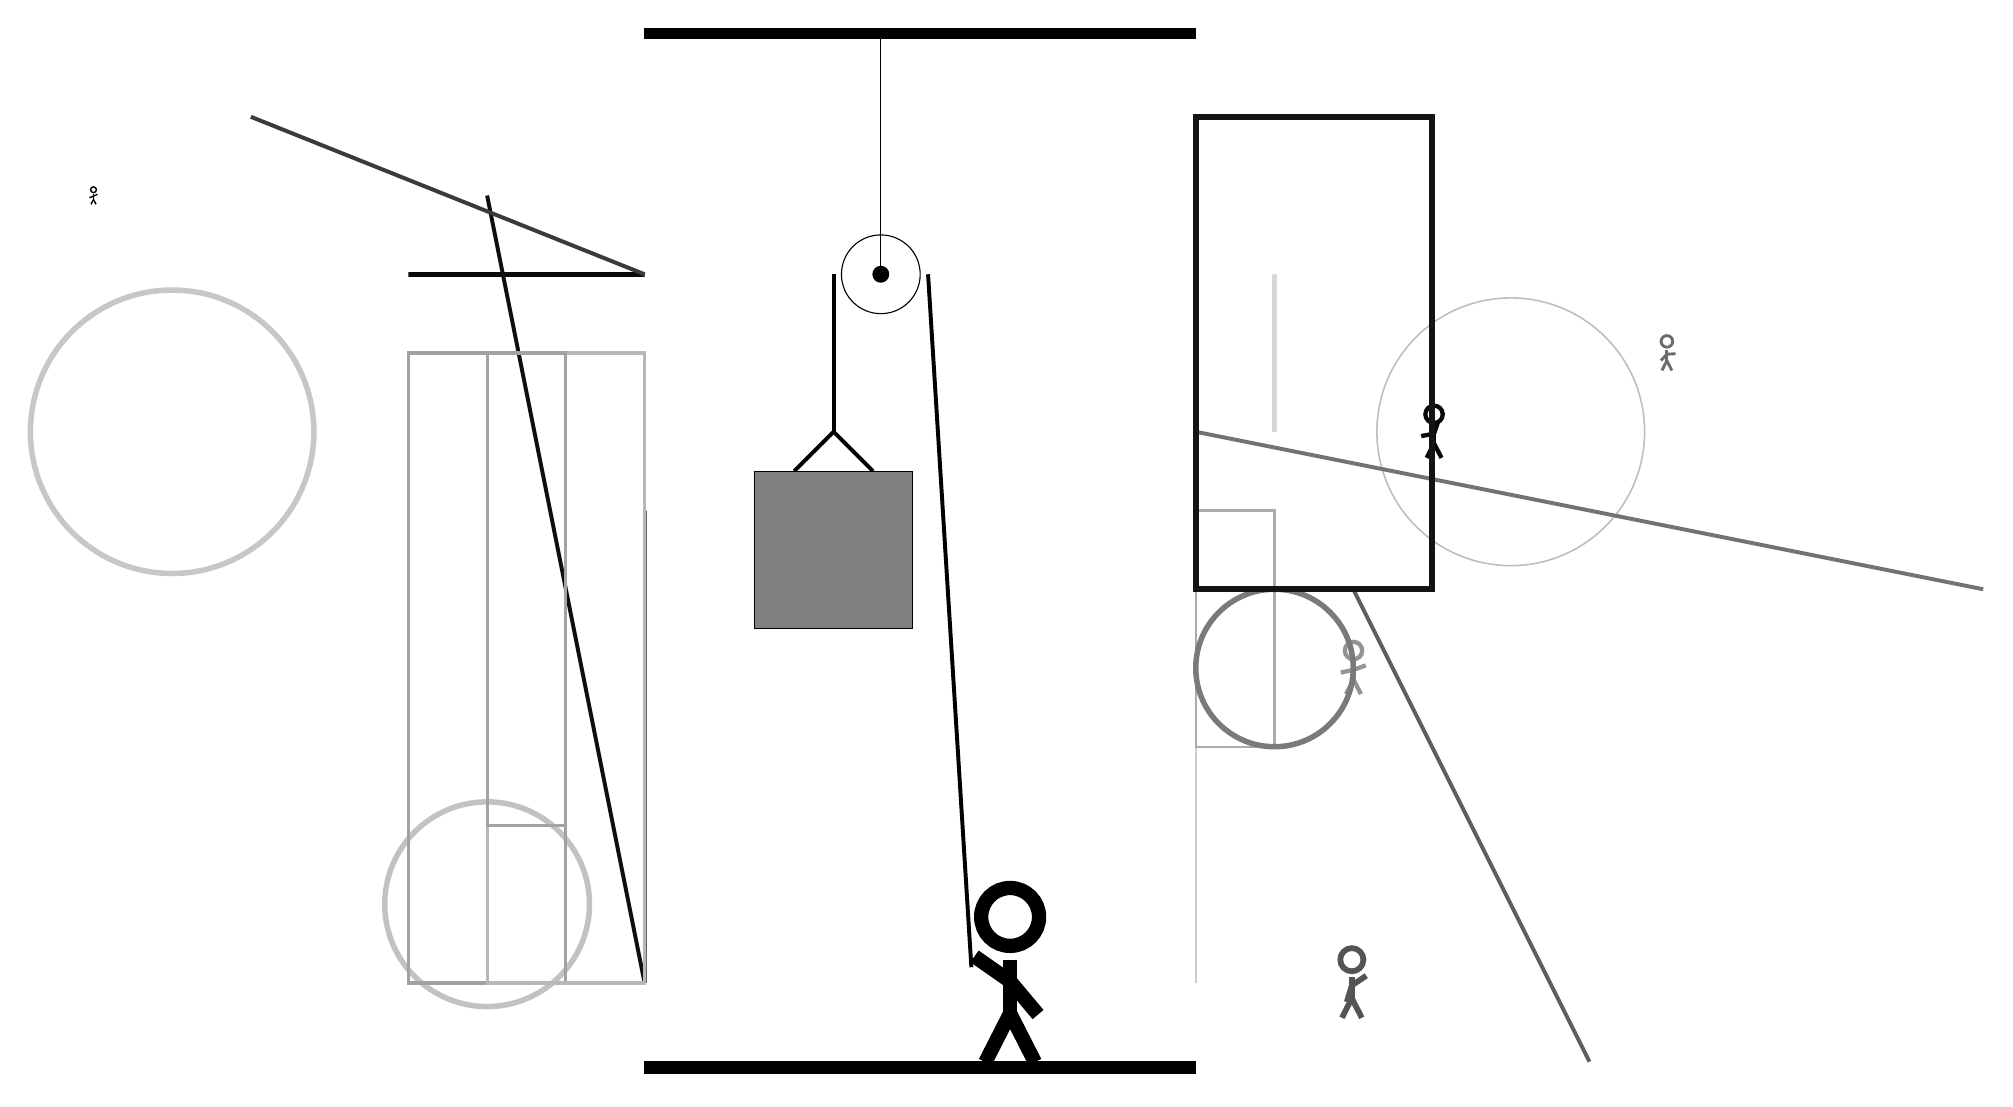
\begin{tikzpicture}
		%%%%% START %%%%%
		
		\draw[fill=black] (-2, 10) rectangle (5, 10.125);
		
		\draw (1, 7) circle (0.5);
		\draw[fill=black] (1, 7) circle (0.1);
		\draw (1, 10) -- (1, 7);
		
		\draw[line width=0.5mm] (-0.1, 4.5) -- (0.4, 5.0) -- (0.9, 4.5);
		\draw[fill=black!50] (-0.6, 4.5) rectangle (1.4, 2.5);
		
		\draw[line width=0.5mm] (0.4, 7) -- (0.4, 5.0);
		\centerarc[line width=0.5mm](1, 7)(0:180:0.6);
		\draw[line width=0.5mm](1.6, 7) -- (2.15, -1.8);
		
		\draw [line width=0.2mm, color=black!26](9, 5) circle (1.7);
		
		\draw[line width=0.7mm, color=black!96] (-2, 7) rectangle (-5, 7);
		\draw[line width=0.2mm, color=black!20] (5, -2) rectangle (5, 6);
		\draw [line width=0.7mm, color=black!22](-8, 5) circle (1.8);
		\draw[line width=0.5mm, color=black!63](7, 3) -- (10, -3);
		\draw [line width=0.7mm, color=black!24](-4, -1) circle (1.3);
		\draw[line width=0.3mm, color=black!33] (6, 1) rectangle (5, 4);
		
		\node[line width=0.6mm, color=black!42] at (7, 2) {\Strichmaxerl[3][12][20]};
		\draw[line width=0.7mm, color=black!16] (6, 5) rectangle (6, 7);
		\node[line width=0.6mm, color=black!58] at (11, 6) {\Strichmaxerl[2][46][4]};
		
		\node[line width=0.4mm, color=black!97] at (8, 5) {\Strichmaxerl[3][11][71]};
		\draw [line width=0.7mm, color=black!52](6, 2) circle (1.0);
		\draw[line width=0.5mm, color=black!94](-2, -2) -- (-4, 8);
		\draw[line width=0.4mm, color=black!37] (-3, 6) rectangle (-5, -2);
		\draw[line width=0.5mm, color=black!55](5, 5) -- (15, 3);
		\node[line width=0.2mm, color=black!99] at (-9, 8) {\Strichmaxerl[1][21][26]};
		
		\draw[line width=0.7mm, color=black!92] (5, 9) rectangle (8, 3);
		
		\draw[line width=0.5mm, color=black!61] (-2, 4) rectangle (-2, -2);
		\draw[line width=0.4mm, color=black!28] (-2, -2) rectangle (-4, 6);
		
		\draw[line width=0.4mm, color=black!36] (-3, 0) rectangle (-4, 6);
		\draw[line width=0.5mm, color=black!77](-2, 7) -- (-7, 9);
		
		\node[line width=0.2mm, color=black!67] at (7, -2) {\Strichmaxerl[4][73][34]};
		
		
		\node at (2.6, -1.9) {\Strichmaxerl[10][-35][-50]};
		
		\draw[fill=black] (-2, -3) rectangle (5, -3.15);
		
		%%%%% END %%%%%
	\end{tikzpicture}
\end{document}